\usetikzlibrary{arrows.meta,shapes,positioning,shadows,trees,decorations.pathmorphing}

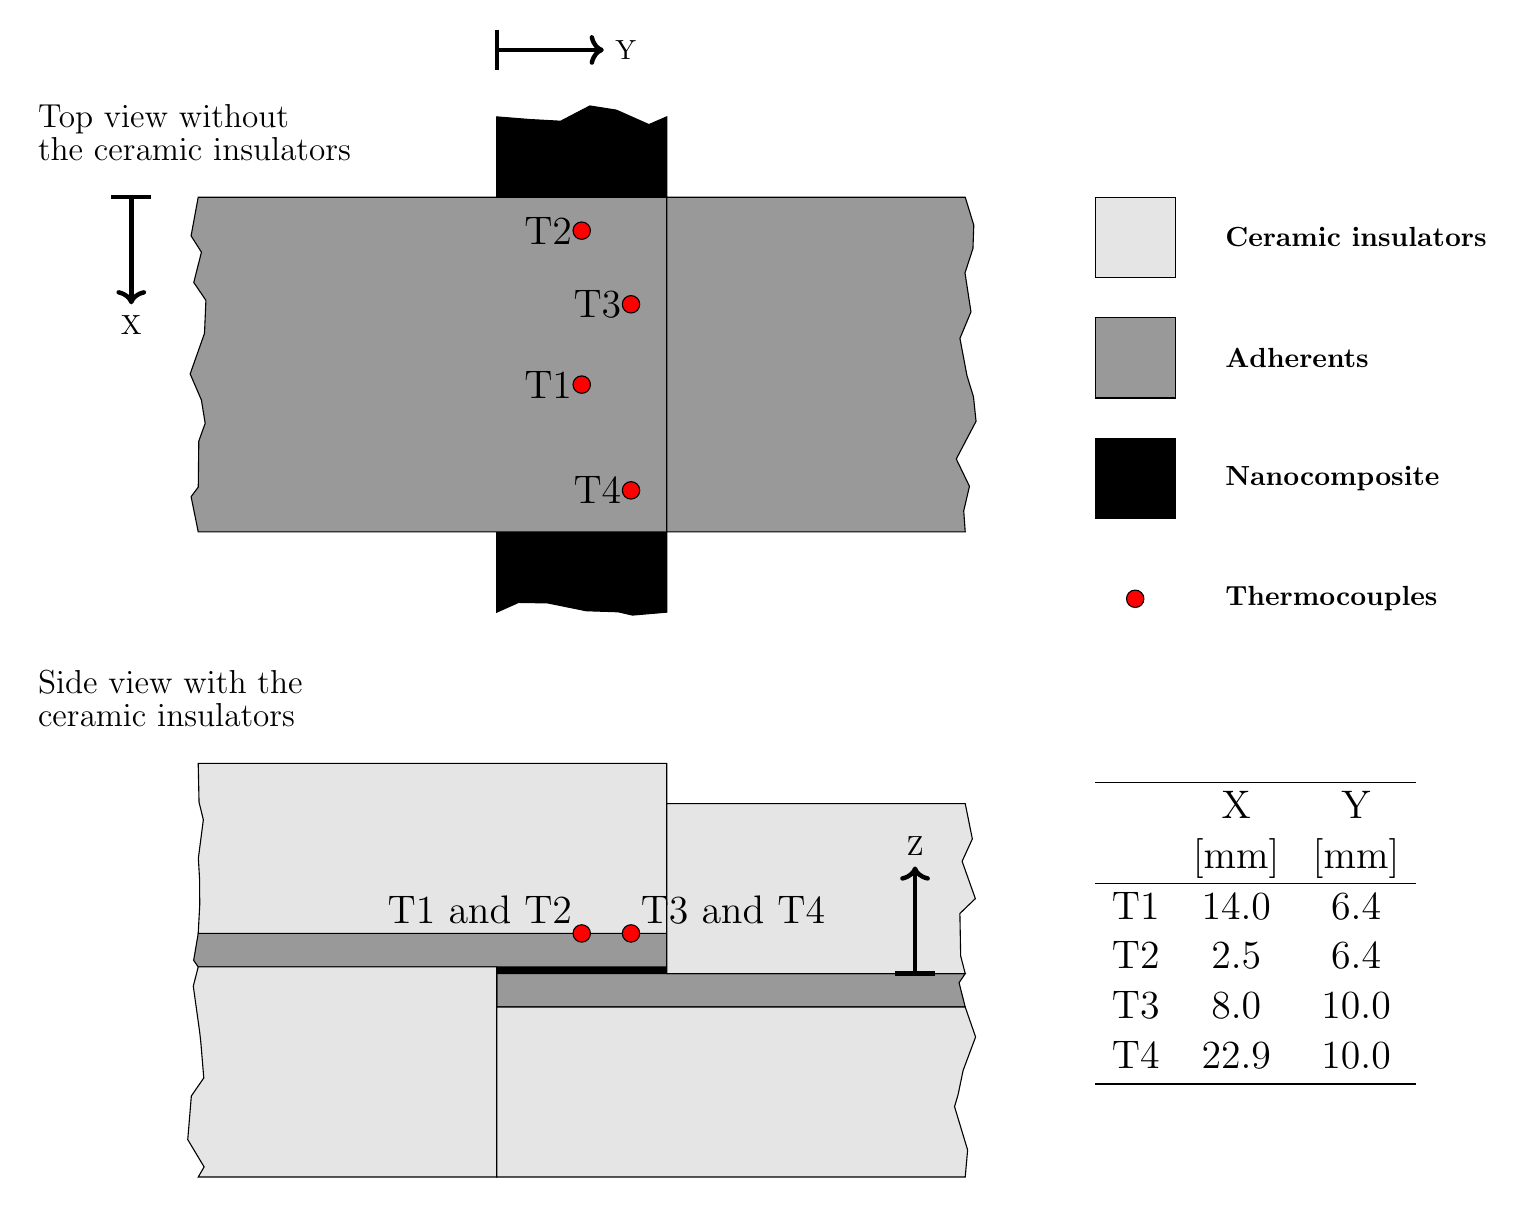
\begin{tikzpicture}[scale=0.17]

%Couleurs
\def \colceramique{black!10}
\def \colcomposite{black!40}

\def \legend{6}

%Définition des dimensions du joint soudé
\def \overlap{12.7}
\def \epceramique{12.7}
\def \epcomposite{2.5}
\def \epnanocomposite{0.5}
\def \longueur{35}
\def \gapfigure{33}
\def \largeursoudure{25}
\def \depassementsoudure{6}
\def \diacercle{0.65}

\def \gaptexte{2}

\def \llegende{8}
\def \distlegende{5}
\def \wlegendtail{3}

%%%Vue du dessus %%%
\draw (-\longueur,\gapfigure+\largeursoudure+\gaptexte) node [above right, align=left]{\large Top view without \\ \large the ceramic insulators};

%Élément chauffant
\draw[black,decoration={random steps, amplitude=4, segment length=10},fill=black] (0,\gapfigure-\depassementsoudure) decorate{-- ++(\overlap,0)} -- ++(0,2*\depassementsoudure+\largeursoudure) decorate{-- ++(-\overlap,0)} -- cycle;

%Adhérent
\draw[black,decoration={random steps, amplitude=4, segment length=10},fill=\colcomposite] 
(0,\gapfigure) -- ++(\longueur,0) decorate{-- ++(0,\largeursoudure)} -- ++(-\longueur,0) -- cycle;
\draw[black,decoration={random steps, amplitude=4, segment length=10},fill=\colcomposite] 
(\overlap,\gapfigure) -- ++(-\longueur,0) decorate{-- ++(0,\largeursoudure)} -- ++(\longueur,0) -- cycle;


%Position du thermocouple
\draw[fill=red] (0.5*\overlap,\largeursoudure+\gapfigure-14) circle (\diacercle) node [left]{\Large T1};
\draw[fill=red] (0.5*\overlap,\largeursoudure+\gapfigure-2.5) circle (\diacercle) node [left]{\Large T2};
\draw[fill=red] (0.79*\overlap,\largeursoudure+\gapfigure-8) circle (\diacercle) node [left]{\Large T3};
\draw[fill=red] (0.79*\overlap,\largeursoudure+\gapfigure-21.9) circle (\diacercle) node [left]{\Large T4};

%%% Vue du côté %%%
\draw (-\longueur,\epceramique+\epnanocomposite+\epcomposite+\gaptexte) node [above right, align=left]{\large Side view with the \\ \large ceramic insulators};

%Éléments chauffants
\draw[black,thick,fill=black] (0,0) -- ++(\overlap,0) -- ++(0,\epnanocomposite) -- ++(-\overlap,0) -- cycle;

%Adhérents
\draw[black,decoration={random steps, amplitude=4, segment length=6},fill=\colcomposite] 
(0,0) -- ++(\longueur,0) decorate{-- ++(0,-\epcomposite)} -- ++(-\longueur,0) -- cycle;
\draw[black,decoration={random steps, amplitude=4, segment length=6},fill=\colcomposite] 
(\overlap,\epnanocomposite) -- ++(-\longueur,0) decorate{-- ++(0,\epcomposite)} -- ++(\longueur,0) -- cycle;

%Céramiques
\draw[black,decoration={random steps, amplitude=4, segment length=10},fill=\colceramique] 
(0,\epnanocomposite) -- ++(-\longueur+\overlap,0) decorate{-- ++(0,-\epceramique-\epnanocomposite-\epcomposite)} -- ++(\longueur-\overlap,0) -- cycle;
\draw[black,decoration={random steps, amplitude=4, segment length=10},fill=\colceramique] 
(\overlap,\epcomposite+\epnanocomposite) -- ++(-\longueur,0) decorate{-- ++(0,\epceramique)} -- ++(\longueur,0) -- cycle;
\draw[black,decoration={random steps, amplitude=4, segment length=10},fill=\colceramique] 
(0,-\epcomposite) -- ++(\longueur,0) decorate{-- ++(0,-\epceramique)} -- ++(-\longueur,0) -- cycle;
\draw[black,decoration={random steps, amplitude=4, segment length=10},fill=\colceramique] 
(\overlap,0) -- ++(\longueur-\overlap,0) decorate{-- ++(0,\epceramique)} -- ++(-\longueur+\overlap,0) -- cycle;

%Position du thermocouple
\draw[fill=red] (0.5*\overlap,\epnanocomposite+\epcomposite) circle (\diacercle) node [above left]{\Large T1 and T2};
\draw[fill=red] (0.79*\overlap,\epnanocomposite+\epcomposite) circle (\diacercle) node [above right]{\Large T3 and T4};

% Système d'axe
\draw[ultra thick, black, ->] (0,\gapfigure+\depassementsoudure+\distlegende+\largeursoudure) -- ++(\llegende,0) node[ right] {Y}; 
\draw[ultra thick, black] (0,\gapfigure+\depassementsoudure+\distlegende+\largeursoudure+0.5*\wlegendtail) -- ++(0,-\wlegendtail); 

\draw[ultra thick, black, ->] (-\distlegende-\longueur+\overlap,\gapfigure+\largeursoudure) -- ++(0,-\llegende) node[below] {X}; 
\draw[ultra thick, black] (-\distlegende-\longueur+\overlap-0.5*\wlegendtail,\gapfigure+\largeursoudure) -- ++(\wlegendtail,0); 

\draw[ultra thick, black, ->] (\longueur-0.75*\distlegende,0) -- ++(0,\llegende) node[ above] {Z}; 
\draw[ultra thick, black] (\longueur-0.75*\distlegende-0.5*\wlegendtail,0) -- ++(\wlegendtail,0); 

%Legend
\begin{scope}[shift={(\overlap+\longueur-0.5*\legend,\gapfigure+\largeursoudure)}]
	\begin{scope}[shift={(0,0)}]
		\draw [black, fill=\colceramique] (0,0) rectangle ++(\legend,-\legend);
		\draw (1.5*\legend,-0.5*\legend) node[right]{{\textbf{Ceramic insulators}}} ;
	\end{scope}

	\begin{scope}[shift={(0,-1.5*\legend)}]
		\draw [black, fill=\colcomposite] (0,0) rectangle ++(\legend,-\legend);
		\draw (1.5*\legend,-0.5*\legend) node[right]{{\textbf{Adherents}}} ;
	\end{scope}

	\begin{scope}[shift={(0,-3*\legend)}]
		\draw [black, fill=black] (0,0) rectangle ++(\legend,-\legend);
		\draw (1.5*\legend,-0.5*\legend) node[right]{{\textbf{Nanocomposite}}} ;
	\end{scope}

	\begin{scope}[shift={(0,-4.5*\legend)}]
		\draw [fill=red] (0.5*\legend,-0.5*\legend) circle (\diacercle);
		\draw (1.5*\legend,-0.5*\legend) node[right]{{\textbf{Thermocouples}}} ;
	\end{scope}

\end{scope}

%Location of thermocouples
\begin{scope}[shift={(\overlap+\longueur+1.5*\legend,0.5*\legend)}]
	\node (thermocouple_location){ \Large
		\begin{tabular}{c c c}
			\hline
			   & X    & Y    \\
			   & [mm] & [mm] \\ \hline
			T1 & 14.0 & 6.4  \\
			T2 & 2.5  & 6.4  \\
			T3 & 8.0  & 10.0 \\
			T4 & 22.9 & 10.0 \\ \hline
		\end{tabular}
	};
\end{scope}



\end{tikzpicture}
